% !TEX root = ../AiiDA_tutorial.tex
%%%%%%%%Inherited from old tutorial
%Task 1 and Taks 2 do not actually need QueryTool, as they inspect a previously defined group.
%The decision to improve it is left to authors of this part
%Taks 3 might be reused but recast to the logic and syntax of QueryBuilder
%%%%%%%%

\section{Queries in AiiDA: The QueryBuilder}
\label{sec:querybuilder}
In this part of the tutorial we will focus on how to query our database using a querying tool for AiiDA called the \textit{QueryBuilder}.
Queries are, very loosely defined, questions to your database.
We will first show you some simple examples and tasks on how to explore your database.
Then we will proceed to a more concrete exercise on the screening of magnetic and metallic perovskites.\\

% In the end we will present some more complicated examples and exercises showing all the possibilities of the QueryBuilder.



%To be deleted or incorporated to the above text:
%
%In the first part of the tutorial, you got an idea of how a single calculation is submitted with AiiDA and how its results can be retrieved, both from the command line and from the \verb|verdi shell|. In this second part of the tutorial, we will instead focus on how to systematically retrieve, query and analyse the results of multiple calculations using AiiDA features. The idea of this part of the tutorial is to screen magnetic and metallic perovskites.
%For time reasons, a set of calculations have already been performed on 57 perovskites, using three different pseudopotential families (LDA, PBE and PBESOL, all from GBRV 1.2~\cite{ref:GBRV}). Each of them was run with the same type of script you tried in Sec.~\ref{sec:qe}, so there is nothing new.
%These calculations have been imported, and they were created by a different user.


%\textcolor{red}{LK: Some text on what is the difference, and to use -A option for all-users with command line}


% If you want to reproduce them, simply put the code of Sec.~\ref{sec:qe} in a Python function, and change the A and B species in a for loop.These calculations are spin-polarised (without spin-orbit coupling), use a Gaussian smearing and perform a variable-cell relaxation of the full unit cell.}

%\textcolor{red}{LK: Some words in QueryBuilder here}


\subsection*{Task 1 - Introduction to QueryBuilder}
\begin{table}[b]
\centering
\begin{tabular}{cc}
\hline
Node \& subclasses & Number in DB \\ \hline
Node                 & 4707 \\
StructureData        & 621 \\
ParameterData        & 1338 \\
KpointsData          & 861 \\
UpfData              & 99 \\
JobCalculation       & 448 \\ \hline
\end{tabular}
\caption{List of some Node subclasses and how many times they occur in our test database.}
\label{fig.types}
\end{table}


In this task we will use the QueryBuilder to do some basic queries and understand our database.
As a first step we should import our querying tool, the \textit{QueryBuilder}.
\begin{pythoncommand}
from aiida.orm.querybuilder import QueryBuilder
\end{pythoncommand}
After the above import, we create our first query.
To do so, we will have to instantiate a QueryBuilder instance:
\begin{pythoncommand}
qb = QueryBuilder()
\end{pythoncommand}
Our query is still empty, we have not yet defined what we want to see.
For example, we will ask for all the nodes of our database.
This is as simple as appending the Node class to the query that we construct.
\begin{pythoncommand}
qb.append(Node)
\end{pythoncommand}
At this point, we can finish our query by asking back all nodes and by typing
\begin{pythoncommand}
qb.all()        # Returns all nodes in the database
\end{pythoncommand}
However, this command will return us all the Nodes directly, which may not be the most wise thing to do
considering that is the biggest family of AiiDA stored objects that we can query.
To understand the size of the result, we can type the following command:
\begin{pythoncommand}
qb.count()      # Returns an integer, the number of nodes in the database
\end{pythoncommand}
% Taking some stuff out do reduce length
%~ If we decide to get a large number of results,
%~ then it is could be better to retrieve them using an iterator and not using the \texttt{.all()} method.
%~ \begin{pythoncommand}
%~ for node, in qb.iterall():
    %~ print node
%~ \end{pythoncommand}
If you are interested to retrieve a subclass of a node, append that specific subclass instead of Node:
\begin{pythoncommand}
StructureData = DataFactory('structure')
qb = QueryBuilder()         # Creating a new QueryBuilder instance
qb.append(StructureData)    # Telling the QueryBuilder instance that I want structures
qb.all()                    # Asking for all the results!
\end{pythoncommand}


\begin{tcolorbox}
\textbf{Exercise:}
\begin{itemize}
\item
Try now to find the number of instances for some subclasses of Node (e.g. StructureData, ParameterData, etc.)
that are stored in your database.
The result should look like \autoref{fig.types}.
Of course, the numbers can be different!
\end{itemize}
\end{tcolorbox}

\textbf{Comment:} If you are familiar with the SQL (Structured Query Language) syntax then you may wonder what the issued SQL command is.
This can be easily seen by typing:
\begin{pythoncommand}
str(qb)
\end{pythoncommand}

\textbf{Comment:}
If you want to get inspired by the available QueryBuilder options you can just press the
\emph{tab} key in an interactive shell (after typing \texttt{qb.}) to see the available options.

\textbf{Comment:} After you run a query, a new \texttt{QueryBuilder} instance
needs to be defined if you want to make a new query.

%%%%%%%%%%%%%%%%%%%%%%%%%%%%%%%%%%%%%%%%%%%%%%%%%%%%%%%%%%%%%%%%%%%%%%%%%%%%%%%%
\subsection*{Task 2 - Projections and filters}

\begin{table}[h]
\begin{center}

\begin{tabular}{ccc} \hline
Operator & Datatype & Example \\ \hline
== & All & \{'==':12\}  \\
in & All & \{'in':['FINISHED', 'PARSING']\} \\ \hline
$>,<,<=,>=$ & floats, integers, dates & \{'$>$':5.2\} \\ \hline
like & Chars & \{'like':'calculation\%'\} \\
ilike & Chars & \{'ilike':'caLculAtioN\%'\} \\ \hline
or & & \{'or':[\{'$<$':5.3\}, \{'$>$':6.3\}]\} \\
and & &  \{'and':[\{'$>$':5.3\}, \{'$<$':6.3\}]\} \\
\hline
\end{tabular}
\end{center}
\caption{Operators currently implemented for all backends.}
\label{tab.filterops}
\end{table}

In database language performing a projection means to extract one or more specific columns from a table. In the AiiDA language this is equivalent to say that we select what properties a query should return out of the queried objects.
For example, we might be interested only in the id of a set of nodes (or their creation date, or any stored value).
To this purpose we should suitably instruct a QueryBuilder object by means of the "project" key.
For example, if we would like to get all the ids of the nodes, we would type the following:
\begin{pythoncommand}
qb = QueryBuilder()
qb.append(Node, project=["id"])
qb.all()
\end{pythoncommand}

\begin{table}[b]
\centering
\begin{tabular}{cc}
\hline
Entity & Properties \\ \hline
Node                 & id, uuid, type, label, description, ctime, mtime \\ \hline
Computer        & \begin{tabular}{@{}c@{}}id, uuid, name, hostname, description,\\ enabled, transport\_type, scheduler\_type\end{tabular} \\ \hline
User        & id, email, first\_name, last\_name, institution \\ \hline
Group          & id, uuid, name, type, time, description \\ \hline
\end{tabular}
\caption{A selection of entities and some of their properties.}
\label{tab.properties}
\end{table}



\begin{tcolorbox}
Please note that if you would like to perform an operation on the \emph{pk} of a node,
you should use the keyword \emph{id} in QueryBuilder queries.
\end{tcolorbox}


Most likely, performing a query implies to select only those elements that fulfill certain criteria.
For example, we might want to select all the calculations that were launched on a specific date.
In database language, this is called "adding a filter" to a query.
A filter is a boolean operator that returns True or False.
\autoref{tab.filterops} lists all operators that we implemented.
A selection of entities and some of their properties that you can use at your projections and filters
can be found at table \autoref{tab.properties}.

If you want to add filters to your query, you simply add the \emph{filters} keyword with a dictionary.
Suppose you want to know the creation date of a structure of which you know the uuid:
\begin{pythoncommand}
qb = QueryBuilder()             # Instantiating a new QueryBuilder
qb.append(
    StructureData,              # I want structures!
    project=["ctime"],          # I'm interested in creation time!
    filters={"uuid": {
            "==":"ace6523a-2019-47c4-98a3-48429265f62c"
        }})                     # I want the structure with this UUID
qb.all()
\end{pythoncommand}
Try it out!
There is also the possibility to combine multiple filters on the same object using the ``and'' or the ``or''
 keyword in the filter section. Let's see an example.
\begin{pythoncommand}
from datetime import datetime, timedelta
qb = QueryBuilder()
qb.append(
    StructureData,
    project=["uuid"],           #  I want to see only the UUID
    filters={"or":[             # First filter is an or statement
            {"ctime": {">":datetime.now() - timedelta(days=12)}},
            {"label": "graphene"}
        ]}
   )
qb.all()
\end{pythoncommand}

In the above example we added an ``or'' keyword between the two filters.
The query return every structure in the database that was created
in the last 12 days or is named "graphene". \\
\textbf{Hints for the exercises:}
\begin{itemize}
\item The operator '>', '<' works with date-type properties with the expected behavior.
\item For your date comparisons you will need to create a \texttt{datetime} object to which you can assign a date of your preference.
 You will have to do the necessary import (\texttt{from datetime import datetime}) and create an object by giving a specific date.
 E.g. datetime(2015, 12, 26). For further information, you can consult the Python's online documentation.
\end{itemize}

\begin{tcolorbox}
\textbf{Exercises:}
\begin{itemize}
\item
Write a query that returns all instances of StructureData that have been created after the 1st of January 2016.
\item
Write a query that returns all instances of Group whose name starts with ``tutorial''.
\end{itemize}
\end{tcolorbox}

% \textbf{Hint 2:} The creation time is stored in a column called \textit{ctime}.

\subsection*{Task 3 - Defining relationships}
In the previous tasks we saw how to select specific entities from AiiDA, how to apply projections
on their properties and how to apply filters.
Moreover, you should know by now how to write complex filters including ``and'' and ``or'' keywords.
In this task we will see how to associate entities by defining relationships among them.

Defining a relationship between two entities is as easy as appending another entity to the QueryBuilder query.
For example, let's look at the following query:

\begin{pythoncommand}
from aiida.orm import Group, JobCalculation
qb = QueryBuilder()
qb.append(JobCalculation,
        tag="mycalculation",            # I tag, so I can refer to this entity later
        project=["*"])                  # I'm asking for ORM instances ("*")
qb.append(Group,                        # Also asking for groups
        group_of="mycalculation",       # I want the calculation to be part of the group
        filters={                       # A filter, the name has to be "pbe_calculation"
            "name":{"==":"pbe_calculation"}
        })
qb.all()
\end{pythoncommand}
This returns all jobs that belong to a Group with the name ``pbe\_calculation''.
The \emph{project=["*"]} returns the AiiDA orm instance (i.e. an instance of \emph{aiida.orm.calculation.job.JobCalculation}).
%
%The graphical representation of the above query can be seen at Figure~\ref{fig:simple_query}.
%~ \begin{figure}[h]
%~ \begin{center}
%~ 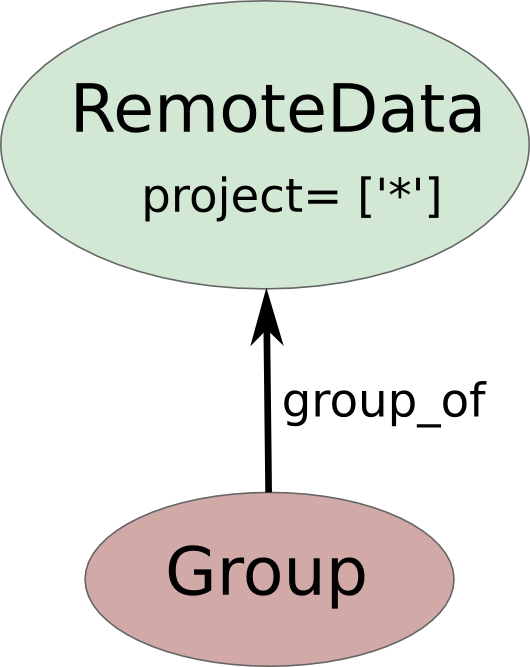
\includegraphics[width=3.5cm]{img/qb_example_1.png}
%~ \end{center}
%~ \caption{Query: Fetch me all the RemoteData that belong to a Group.}
%~ \label{fig:simple_query}
%~ \end{figure}
%
%
There are few details that we should remember from the above query:
\begin{itemize}
\item We \emph{append} to the QueryBuilder instance new entities, and specify how they linked
to previous entities with keywords (``input\_of'', ``output\_of'', ``group\_of'').
The possible relationship keywords can be seen at table~\ref{table:join_rel}.
\item Therefore, we have to \emph{tag} the entities that we want to reference.
We pass these tags along with the keyword, to define a relationship.
\end{itemize}


\begin{table}
	\begin{center}
		\begin{tabular}{l l l l}
		Entity from	& Entity to	& Relationship & Explanation\\ \hline\hline
		Node & Node & input\_of & One node as input of another node\\
		Node & Node & output\_of & One node as output of another node\\
		Node & Node & ancestor\_of & One node as the ancestor of another node\\
		Node & Node & descendant\_of & One node as descendant of another node\\\hline
		Group & Node & group\_of & The group of a node\\
		Node & Group & member\_of & The node is a member of a group\\\hline
		Computer & Node & computer\_of & The computer of a node\\
		Node & Computer & has\_computer & The node of a computer\\\hline
		User & Node & creator\_of & The creator of a node is a user\\
		Node & User & created\_by & The node was created by a user\\
		\end{tabular}
		\caption{Available relationships}
		\label{table:join_rel}
		\end{center}
	\end{table}



\begin{tcolorbox}
\textbf{Exercise:}
\begin{itemize}
	\item Write a query that returns all the StructureData that are an input of a JobCalculation.
\end{itemize}
More (optional) exercises on entity relationships can be found at the appendix.
\end{tcolorbox}


\subsection*{Task 4 - Attributes and extras}
Node and its subclasses have properties stored in key/value format.
These are called \emph{attributes} and \emph{extras} and can be used in filters and projections as the other properties that we have seen previously.

Let's project the value of the property \emph{attributes.energy\_smearing}.
\begin{pythoncommand}
qb = QueryBuilder()
qb.append(
        ParameterData,
        project=["attributes.energy_smearing"]
    )
qb.all()
\end{pythoncommand}
The above query takes the attributes properties of every ParameterData and searches for a
key called energy\_smearing. If that key is found, the value is projected,
otherwise the value is None.  Try it out!
% Of course, searching inside key/values can go as deep as needed.
% E.g. you can project on attributes.a.b.c which will correspond to a property \texttt{\{..., "a": \{... "b": \{... "c": "val" ...\} ...\}, ...\}} % THIS STUFF DOES NOT CORRESPOND TO OUTPUT
~\\~\\
% textcolor{blue}{SZ: What happens with lists?}

\textbf{Hints for the exercises:}
\begin{itemize}
\item If you are unsure about the key of the node that you would like to project, you can print all the attributes of a specific node to get some inspiration. This can be done by calling the \texttt{.get\_attrs()} method of a specific node.
\item The pseudopotentials are stored in AiiDA in with the help of the ORM class UpfData. The element that the pseudopotential correspond to is stored in the \emph{attributes.element} property.
\end{itemize}

\begin{tcolorbox}
\textbf{Exercises:}
\begin{itemize}
	\item Print all the attributes of any ParameterData node stored in your database.
	\item Write a query that checks if you have the pseudopotentials for the element \textit{Si}. Do the same for \textit{C}.
\end{itemize}
More (optional) exercises on attributes and extras can be found at the appendix.
\end{tcolorbox}

%\textcolor{blue}{SZ: Distinct doesn't seem to work on attributes.}

\subsection*{Task 5 - A small ``high-throughput'' analysis}

\begin{figure}[!b]
 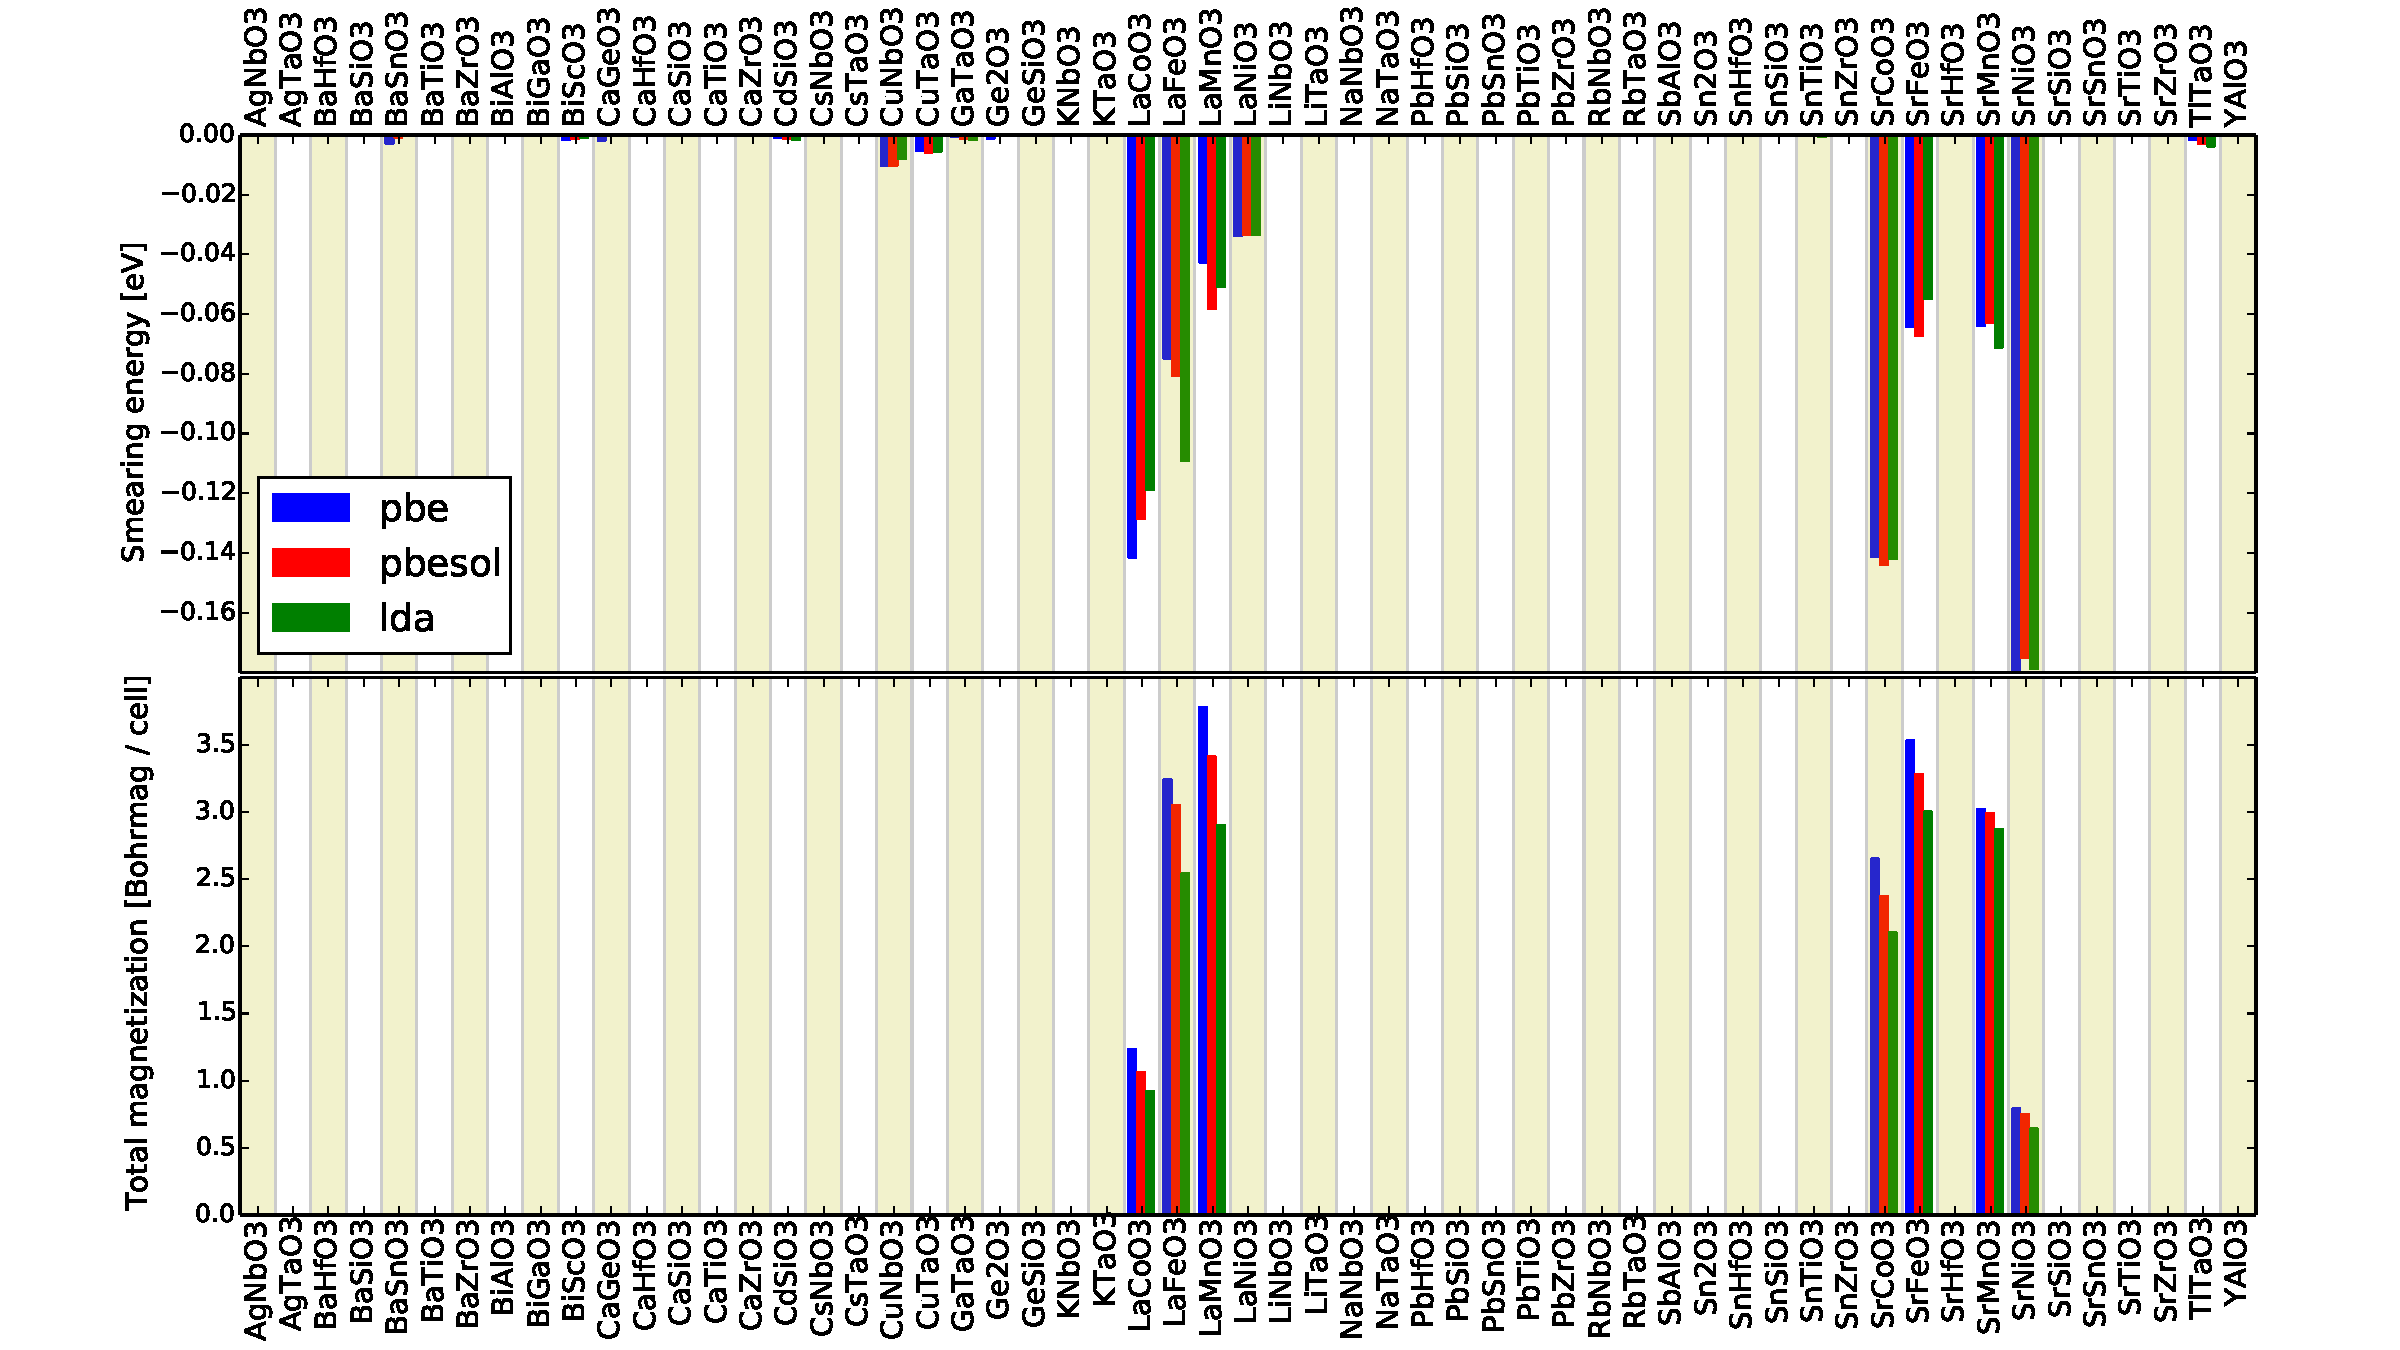
\includegraphics[width=\linewidth]{img/magnetization_smearing_perovskites.pdf}
 \caption{The contribution from the smearing to the total energy (upper) and the magnetization per unit cell (lower)
 in all the perovskites analyzed and for three different pseudopotential families.}
 \label{fig:barplot_perov}
\end{figure}
%
%In the first part of the tutorial, you got an idea of how a single calculation is submitted with AiiDA and how its results can be retrieved, both from the command line and from the \verb|verdi shell|.
In this part of the tutorial, we will focus on how to systematically retrieve, query and analyze the results of multiple calculations using AiiDA.
We know you're able to do this yourself, but to save time, a set of calculations have already been done with AiiDA for you on 57 perovskites,
using three different pseudopotential families (LDA, PBE and PBESOL, all from GBRV 1.2~\cite{ref:GBRV}).
These calculations are spin-polarized (without spin-orbit coupling),
use a Gaussian smearing and perform a variable-cell relaxation of the full unit cell.
The idea of this part of the tutorial is to ``screen'' for magnetic and metallic perovskites in a ``high-throughput'' way.

As you learned in the first part of the tutorial, AiiDA allows to organize calculations in groups.
Once more check the list of groups in your database by typing

\begin{bashcommand}
 verdi group list
\end{bashcommand}

The calculations needed for this task were put in three different groups whose names start with "tutorial\_" (one for each pseudopotential family).
The main task is to make a plot showing, for all perovskites and for each pseudopotential family,
the total magnetization and the $-TS$ contribution from the smearing to the total energy.
An example is shown in \autoref{fig:barplot_perov}.

\subsubsection*{Preparing the analysis}
Let us now guide you through the definition of the query that allows you to retrieve the relevant data.\\~\\
\textbf{Hint for the exercise}:
\begin{itemize}
\item To select multiple names in a filter your filter-dictionary should look like
\begin{pythoncommand}
qb.append(Group, filters={"name": {"in": ["name1","name2","name3"]}})
\end{pythoncommand}
\end{itemize}

\begin{tcolorbox}
\textbf{Exercise:}\\~\\
Please perform the following steps
\begin{enumerate}
\item Write a query to retrieve the three groups and project the respective names.
\item Extend the query to the PwCalculation nodes that are members of the selected groups.
\item Extend the query so that also the chemical formula of the input structure of each calculation is returned.
For simplicity the formulas have been added in the extras of each structure node under the key \textit{"formula"}.
The chemical formula of a StructureData node can also be accessed by the method \cmd{structure.get\_formula()}
\item Every successful PwCalculation has in output a ParameterData instance that stores the results as key-value pairs.
You can find these pairs among the attributes.
To facilitate querying, the parser takes care of storing values always in the same units, and these are documented.
For convenience, the units are also added as key/value pairs (with the same key name, but with \cmd{\_units}  appended).
% Load a ParameterData node (ex. pk=3516) and find the keys that you are interested in by typing:
% \begin{pythoncommand}
% node.get_attrs()
% \end{pythoncommand}
Extend the query so that also the output ParameterData of each calculation is returned.
Project only the attributes relevant to your analysis (like smearing energy, ...).
\end{enumerate}
\end{tcolorbox}

\subsubsection*{Running the query and plotting the results}

% We will now get into a small high-throughput analysis of a larger number of PwCalculations.
% The goal is to extend the above query so that you project also on the resulting magnetization, smearing, and group name of the group they belong to.
Now that your query is ready just run it:
\begin{pythoncommand}
 res = qb.dict()
\end{pythoncommand}
The above results returns a list of dictionaries.
In order to be able to plot the data that you have retrieved a script called \texttt{plot\_calculation\_results.py}
was provided to you. This script reads an input text file containing the data and produces a plot similar to \autoref{fig:barplot_perov}.

You should prepare this input text file in the following format,
formatting the data present in \texttt{res}.
Each row in the input file represents one calculation and contains the following informations separated by a comma:

\begin{enumerate}
\item The structure formula.
\item The name of the pseudo family. Remove the tutorial\_ substring from the name if it bothers you.
\item The smearing energy
\item The unit used for the smearing energy.
\item The magnetization.
\item The unit of the magnetization.
\end{enumerate}

As an example, the first three lines can look like:
\begin{bashcommand}
Sn2O3,  pbesol, -1.95921960844e-05,  eV,  0.0,  Bohrmag / cell
CaSiO3,    pbe,                0.0,  eV,  0.0,  Bohrmag / cell
CuNbO3,    pbe,    -0.010202636111,  eV,  0.0,  Bohrmag / cell
\end{bashcommand}

%Once this is done, you can read the this file with the provided script.


\iffalse
You should be able to print the data in the desired format with about ten lines of python code. In case you are not very familiar with python, you may take inspiration from the following snippet:

\begin{pythoncommand}
with open("res.txt","w") as fout:
  for row in res:
    formula = row["structure"]["extras.formula"]
    magnetization = row["results"]["attributes.total_magnetization"]
    magnetization_units = row["results"]["attributes.total_magnetization_units"]
    smearing = row["results"]["attributes.energy_smearing"]
    smearing_units = row["results"]["attributes.energy_smearing_units"]
    pseudo_family = row["group"]["name"].replace("tutorial_", "")
    str_row = ", ".join(
            map(str, (formula, pseudo_family,
            smearing, smearing_units, magnetization, magnetization_units
        ))
    	)
    fout.write("{}\n".format(str_row))

\end{pythoncommand}
\fi


If you are producing the desired output, write that output to a file (here we will call it \texttt{res.txt}).
If you are using \emph{jupyter}, you can plot the files and see the results directly in the browser. First, in a cell, do
\begin{pythoncommand}
cd ~/tutorial_scripts/
\end{pythoncommand}
to go to the right folder, and then in the following cell type:
\begin{pythoncommand}
%pylab inline
import plot_calculation_results
plot_calculation_results.plot_results('../res.txt')
\end{pythoncommand}
(possibly replacing \texttt{../res.txt} with the correct location of the file).

Otherwise, if you are not using \emph{jupyter}, to plot your data just go in the shell and change directory to the subfolder \texttt{tutorial\_scripts}. Then type in the shell
\begin{bashcommand}
python plot_calculation_results.py ../res.txt
\end{bashcommand}
(or replace \texttt{../res.txt} with the correct location of the \texttt{res.txt} file). The \texttt{plot\_calculation\_results.py} file is already provided to you among the scripts given to you for the tutorial, in the \texttt{tutorial\_scripts} folder. If everything is right, you should get a plot similar to \autoref{fig:barplot_perov}.
You can also pass an option to store the output as a plot on a file:
\begin{bashcommand}
python plot_calculation_results.py res.txt -o myresult.pdf
\end{bashcommand}


\begin{tcolorbox}
\textbf{Exercise:}
\begin{itemize}
\item Look at the plot that you produced. Which of the perovskites are metals?
\end{itemize}
\end{tcolorbox}


%~ \begin{pythoncommand}
%~ qb = QueryBuilder()
%~ qb.append(StructureData, project="*")
%~ qb.append(Calculation, tag="calc")
%~ qb.append(
		%~ ParameterData,
		%~ project="attributes.energy",
		%~ filters={"attributes.energy":{"<=":0}}
	%~ )
%~ qb.append(Group, group_of="calc")
%~
%~ for structure, energy in qb.iterall():
    %~ print structure.get_formula(), energy
%~ \end{pythoncommand}


%~ Figures~\ref{fig:barplot_mag} and~\ref{fig:barplot_smearing} show the plots you should obtain (note that in Fig.~\ref{fig:barplot_smearing} we actually plotted $|-TS|=TS$ since $-TS$ is negative for all the species studied).

%

%\begin{figure}[tb]
% 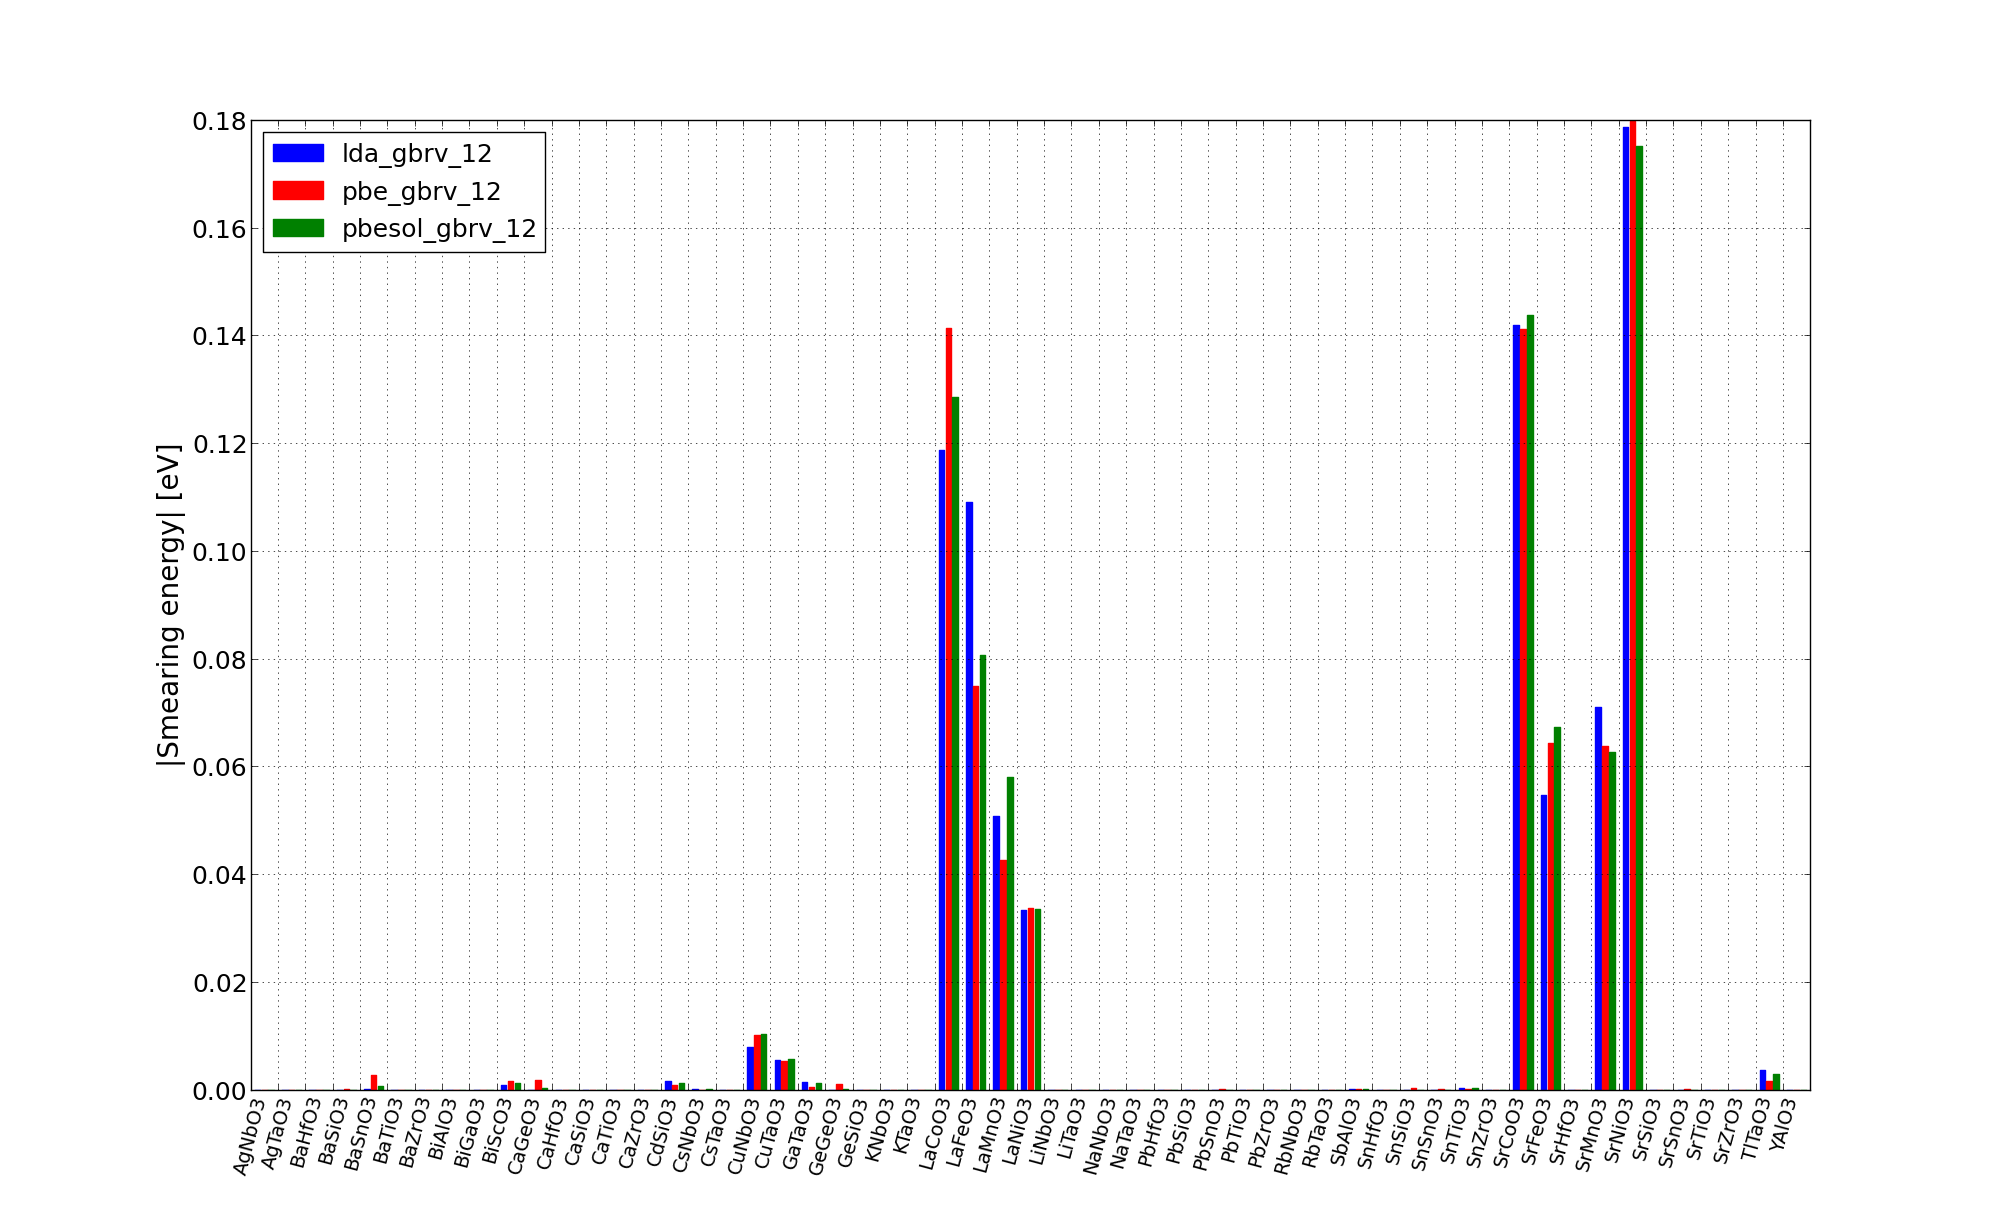
\includegraphics[width=\linewidth]{img/smearing_energy_vs_perovskites_allpseudo_Gaussian_0p02.png}
% \caption{$-TS$ contribution to the total energy (in absolute value, since it is actually negative for all species) from the smearing, for all the perovskites analyzed and for three different pseudopotential families\label{fig:barplot_smearing}.}
%\end{figure}
%
%Two python scripts can help you doing this (you can find them in the subfolder \texttt{$\sim$/tutorial\_scripts}):
%\begin{itemize}
%\item \texttt{get\_pks.py}: gives a list of pk numbers for a given group, possibly filtering also for those perovskites with given ``A"" and/or ``B"" species.
%
%Use it from the command line in the following way:
%\begin{bashcommand}
% ./get_pks.py <group_name> -A <A_element> -B <B_element>
%\end{bashcommand}
%This script prints on output the list of pks (first column) and chemical formulas (second column) of the perovskite(s). The \cmd{-A} and \cmd{-B} options are optional.
% \item \texttt{get\_info.py}: prints several information about a given calculation.
%
%You can use it (from a terminal) with the command
%\begin{bashcommand}
% ./get_info.py <pk_number>
%\end{bashcommand}
%\end{itemize}
%%
%We suggest that you give a look to the content of the scripts we provide, to understand what they do. To prepare the plots, you can either create your own python script taking inspiration from the two scripts that we provide, or (if you do not want to write a Python script, but rather use bash commands) you can simply use the provided scripts as they are.
%Note also that if the graphical plotting software is too slow to load over SSH, you can create a text data file on the remote machine, then copy the data on your computer, and prepare the plot there (you can use any software you like: gnuplot, xmgrace, or even simply Excel).


%~ \subsection*{Task 5.2}
%~ We chose five calculations (using the PBEsol pseudopotential family) of five different representative perovskites, for which we plotted the $-TS$ contribution as a function of the Kohn-Sham band-gap. The resulting plot is shown in \cref{fig:smearing_vs_bandgaps}. \begin{tcolorbox}
%~ Use this plot and the plots you obtained for the smearing energy of all perovskites, to define a criterion to distinguish which compounds are metals and which ones are insulators.
%~ \end{tcolorbox}

%
%\begin{figure}[tb]
% \centering
% 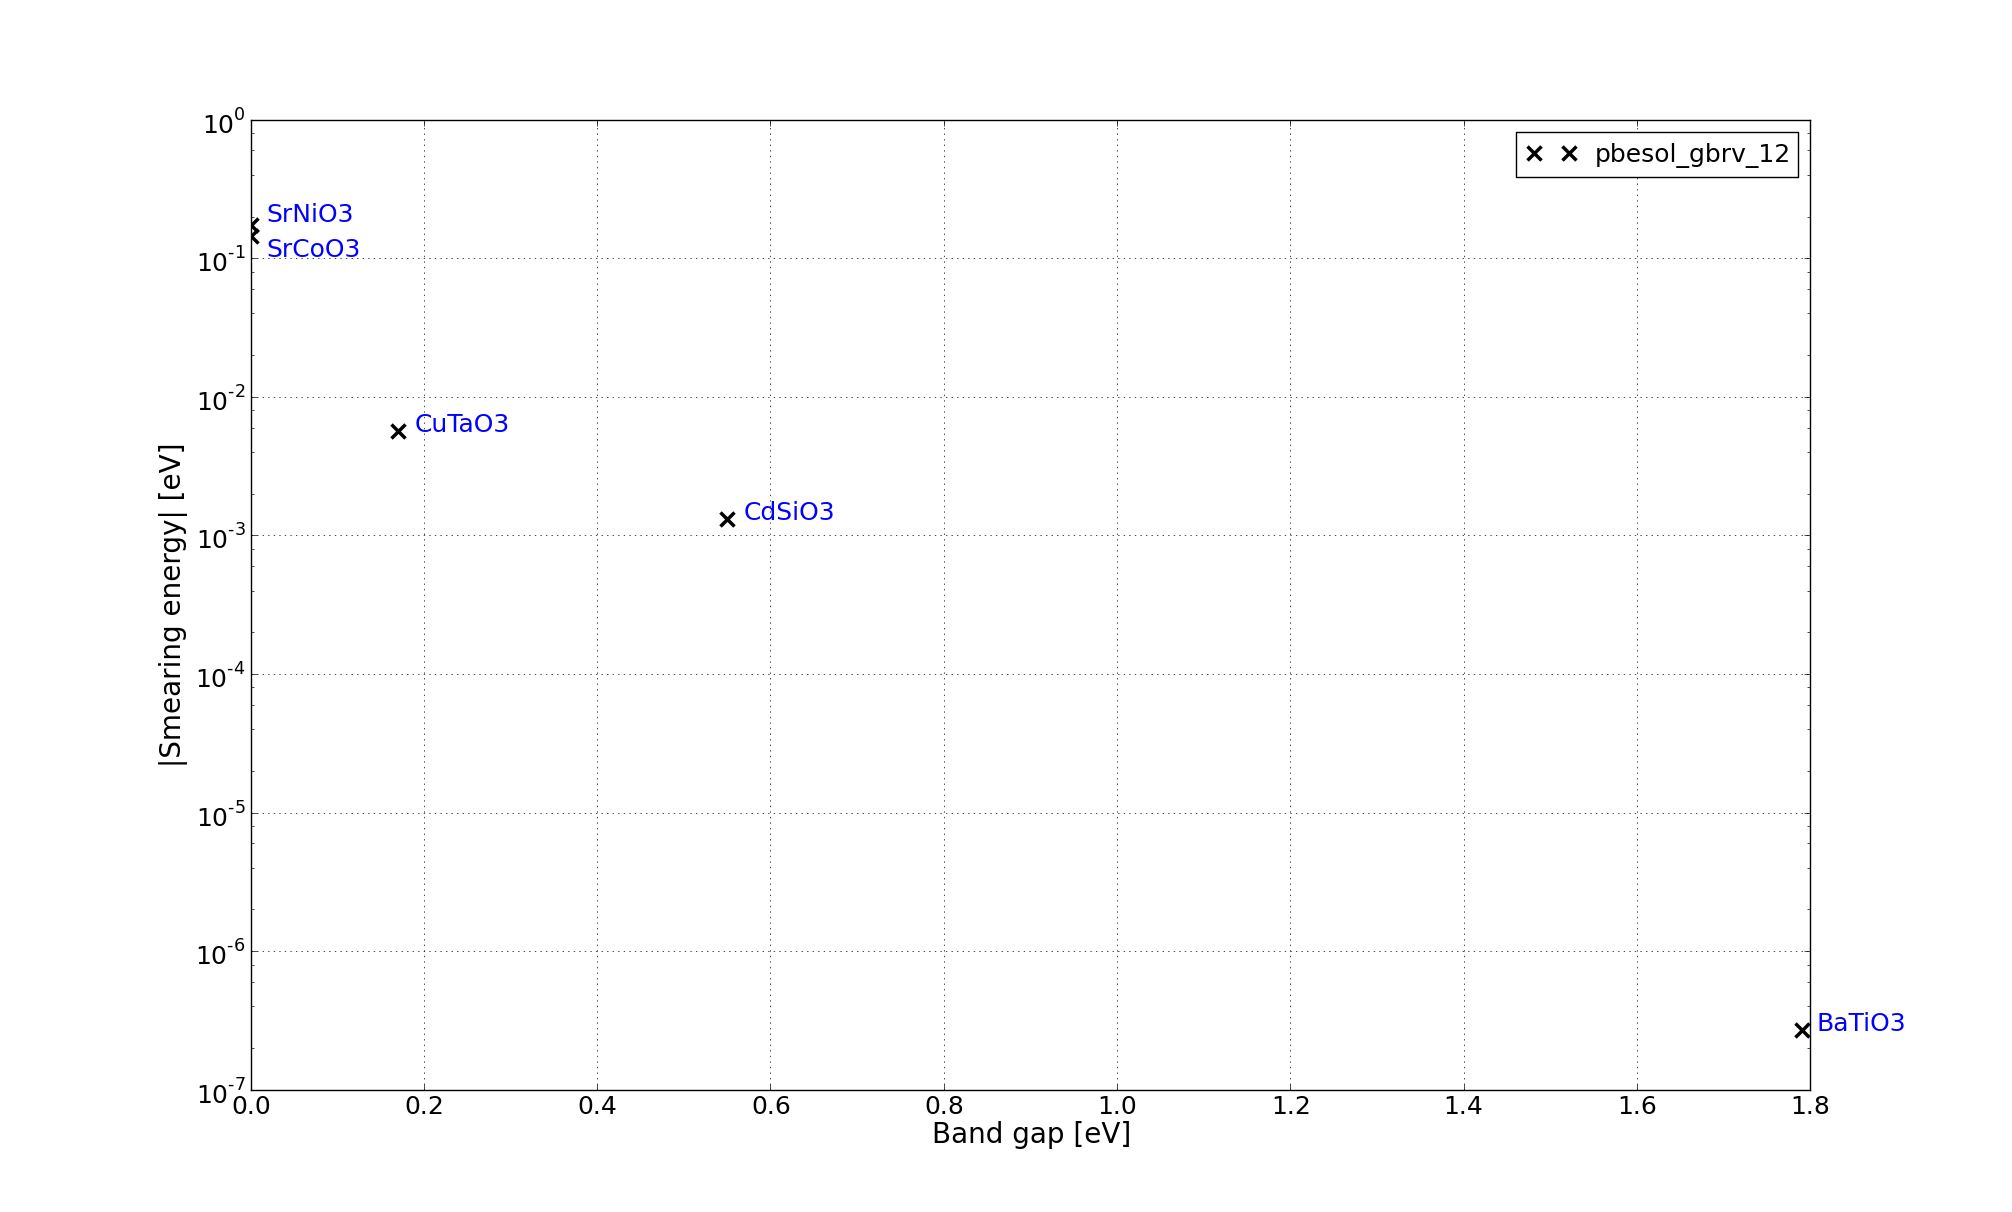
\includegraphics[width=0.7\linewidth]{img/smearing_energy_vs_bandgap_Gaussian_0p02.png}
% \caption{$-TS$ contribution (in absolute value) vs. Kohn-Sham band-gap for five selected perovskites, using the pseudopotentials with PBEsol functional\label{fig:smearing_vs_bandgaps}.}
%\end{figure}
%

%~ \subsection*{Task 5.3}
%~ Finally, we want to print the list of perovskites which are metals according to the criterion we defined, and those that are magnetic. To this aim, we can use the \emph{QueryBuilder} that helps you making easy queries to the database, without the need of knowing the SQL language.



%~ \begin{tcolorbox}
%~ Do another query to find out metallic perovskites according to the criterion on the smearing energy you found above. Check that your query results are consistent with the plots you did at the beginning of the exercise.
%~ \end{tcolorbox}
